% Default course lecture note template by asp 
\documentclass[letterpaper]{article}
\usepackage[utf8]{inputenc}
\usepackage[T1]{fontenc}
\usepackage[english]{babel}
\usepackage[top=3cm, bottom=3cm, left=3.85cm, right=3.85cm]{geometry}
\usepackage[onehalfspacing]{setspace}
\usepackage{hyperref}
\usepackage{amsmath,amsthm,amssymb,wasysym,fdsymbol,marvosym}
\usepackage{graphicx}
\usepackage[usenames,dvipsnames]{color}

\newcommand{\ftwo}{\mathbb{F}_2}
\newcommand{\fttwo}{\mathbb{F}_{32}}
\newcommand{\ftttwo}{\mathbb{F}_{1024}}
\newcommand{\binrep}[1]{\left\{#1\right\}}
\newcommand{\vc}[1]{\texttt{#1}} % volvelle character

\title{
    \emph{The} codex32 \emph{Mathematical Companion}
}
\author{Pearlwort Snead}
\date{
    %currentdate %gitcommit
}

\begin{document}
\maketitle
\tableofcontents

% Actual content start
\section{Mathematical Preliminaries}

In this first section we give a crash course in field theory. Readers familiar
with this material should have no problem skipping or skimming this section,
at least up to Section~\ref{sec:sss}.
Readers who are completely unfamiliar with this material are unlikely to be
able to follow the condensed exposition, and are encouraged to consult
standard algebra textbooks (e.g.~the one by Dummit and Foote) or Wikipedia.

\subsection{Fields and $\ftwo$}
Consider the integers modulo 2. This is a set consisting of two equivalence
classes, the evens and the odds, which hereafter we will refer to as 0 and 1.
This set is a \textbf{field}, which means that when we define addition and
multiplication in the obvious way, it satisfies the following axioms:
\begin{enumerate}
\item The set is closed under addition; addition is associative, commutative,
has an identity element 0, and all elements have additive inverses. In other
words it is an \textbf{abelian group} under addition.
\item Similarly it is an abelian group under multiplication, with identity 1.
\item The \textbf{distributive law} holds, which means that $a(b + c)$ always
equals $ab + ac$.
\end{enumerate}

We refer to this field as $\ftwo$. For any field, we refer to its nonzero
elements as the \textbf{multiplicative group} of the field. We observe that
the multiplicative group of $\ftwo$ has only the identity element.

\subsection{Polynomial Rings}

Since $\ftwo$ has only two elements, it is hard to do interesting algebra on
it. But it is a fact that, by adjoining a formal symbol $x$ to a field, we
can obtain a much bigger (in fact, countably infinite) set of \emph{polynomials}
in $\ftwo$. We denote this set $\ftwo[x]$ and call it the \textbf{polynomial
ring} of the field.

Formally, the set of polynomials is defined as

\[ \left\{ \sum_{i=0}^n a_{i}x^i : n\in\mathbb{N}\cup\{0\}, a_i\in \ftwo  \right\} \]

A ring, for our purposes, is defined the same way as a field except that we do
not require multiplication to be invertible. It is easy to check that the
polynomial ring, endowed with addition and multiplication in the obvious ways,
is in fact a ring.

For a polynomial of the form $\sum_{i=0}^n a_{i}x^i$ with $a_n\neq0$ we refer to $n$ as the
\textbf{degree} of the polynomial. It is an elementary fact that the product
of polynomials has degree equal to the sum of the degrees of the factors.

We refer to polynomials of degree 0 is \textbf{constant polynomials}. It is
also a fact that a polynomial has a multiplicative inverse, i.e.~it is a
\textbf{unit}, if and only if it is nonzero constant.

If whenever a polynomial $r$ is written as the product of two polynomials $r=pq$,
either $p$ or $q$ is a unit (i.e.~degree 0), then we say $r$ is \textbf{irreducible}.

\subsection{Quotient Fields}

Just like we can consider the integers modulo some integer $n$, thus obtaining
$n$ equivalence classes which inherit (roughly) the original ring structure of
the integers, we can consider a polynomial ring modulo some polynomial $p$. In
this case, we will get $m^n$ equivalence classes, where $m$ is the number of
elements in the underlying field and $n$ is the degree of the polynomial.

We call the set of equivalence classes a \textbf{quotient ring}, and its addition
and multiplication are defined in the obvious way.

Just like in the integer case, if our polynomial $p$ can be factored into
nonconstant polynomials as $p=p_1p_2$, their images in the quotient ring will
be nonzero but satisfy $p_1p_2 = 0$. In other words they are \textbf{zero
divisors} and imply that multiplication in the ring is not invertible.

We do not like zero divisors, so from here on out we will be sure to mod out
our polynomial ring only by irreducible polynomials. It is a fact that the
resulting quotient ring will then be a field, and we term it a \textbf{quotient
field}. It is a fact that $x^5 + x^3 + 1$ is irreducible in $\ftwo$, so that
$\ftwo/(x^5 + x^3 + 1)$ is a quotient field with 32 elements. The original
field, $\ftwo$, we refer to as the \textbf{base field}.

In this field the object $x$ is a field element with a distinct identity and
algebraic properties, so we rename it $\alpha$ to preserve the symbol $x$ to
be an indeterminate used for writing polynomials.

For any element $\delta$ in the quotient field, we can talk about its
\textbf{minimal polynomial} over the base field. This is a monic polynomial
(one whose highest-degree coefficient is 1) over the base field, of minimal
degree, such that $\delta$ is a root when the polynomial is considered over
the extension field. It is a fact of field theory that for any element
$\delta$, a unique such minimal polynomial exists. We sometimes refer to the
\textbf{degree} of $\delta$ as being the degree of its minimal polynomial.

Whenever we walk about minimal polynomials or degrees of field elementns, it
is understood that we are considering the elements relative to some base field,
but it will always be clear from context what this base field is, so that we
can use these terms unambiguously.

It is a fact that, for this specific polynomial, that $\alpha$ is a
\textbf{generator} of the quotient field, meaning that the field in its entirety
is equal to
\[ \left\{ \alpha^i : i \in \{0,1,\ldots,30\} \right\} ~\cup~ \left\{ 0 \right\}. \]

We observe that the order of the multiplicative group is 31, a prime, and therefore
every element of the group except 1 is a generator of the group. Furthermore there
are no nontrivial proper subgroups. These are elementary facts of group theory.

We refer to this new field as $\fttwo$. It is fact of field theory that all
groups with 32 elements are isomorphic to this one, which justifies the name.
But bear in mind that, for our purposes, the field was constructed as $\ftwo[x]/
(x^5 + x^3 + 1)$ and has a distinguished generator $\alpha$ which is a root
of that polynomial.

\subsection{Vector Spaces}

We observe that $\fttwo$ is a \textbf{vector space} over $\ftwo$. A vector
space $V$ over a field $\mathbb{F}$ is defined by the following axioms:

\begin{enumerate}
\item $V$ is an abelian group with operation $+$ and identity $0_V$.
\item $(a + b)v = av + bv$ and $a(u + v) = au + av$ for all $a,b\in \mathbb{F}$ and
$u,v\in V$.
\end{enumerate}

We refer to a finite sum of the form $\sum_i f_{i}v_i$ with $f_i\in \mathbb{F}$ and
$v_i\in V$ as a \textbf{linear combination}. We observe that every element
of $\fttwo$ is a linear combination of the elements $\{1,\alpha,\alpha^2,
\alpha^3,\alpha^4\}$, and that no smaller set of elements has this property.
We call such a set a \textbf{basis} for $\fttwo$.

\subsection{Lagrange Interpolation and Shamir's Secret Sharing\label{sec:sss}}

Let $\mathbb{F}$ be a field and $p$ a polynomial of degree $n$ in $\mathbb{F}[x]$. It is a
standard theorem of algebra that $p$'s value on all points of $\mathbb{F}$ is
implied by its values on any $n+1$ distinct points.

As discovered by Edward Waring in
1779\footnote{Waring, Edward (1779). ``Problems concerning interpolations''.
\emph{Philosophical Transactions of the Royal Society}. 69: 59–67.
doi:10.1098/rstl.1779.0008.},
and later by Joseph-Louis Lagrange in 1795\footnote{Lagrange, Joseph-Louis (1795).
``Leçon Cinquième. Sur l'usage des courbes dans la solution des problèmes''.
\emph{Leçons Elémentaires sur les Mathématiques}}\footnote{Both citations taken
from Wikipedia's ``Lagrange Interpolation'' page, March 2023.},
it is actually possible to compute
the value of a polynomial at a field element $x$ explicitly in terms of
its values at $n$ given distinct points $x_i$.

Specifically, suppose that $p(x_i) = y_i$. Then
\begin{equation}
 p(x) = \sum_{i=1}^{n+1} y_i \ell_i(x) \label{eq:linterp}
\end{equation}
where $\ell_i$ is determined entirely by the $x_i$'s, as
\[ \ell_i(x) = \prod_{j\neq i} \frac{x - x_j}{x_i - x_j} \]

There are several very interesting observations to be made here:
\begin{enumerate}
\item First, for a fixed set of $x_i$'s, we see that the vector space of
$n$-degree polynomials over $\mathbb{F}$ is spanned by the set $\{\ell_i(x)\}$. Since
there are $n+1$ polynomials and this space has dimension $n+1$ (an obvious
basis for it is $\{ 1,x,x^2,\ldots,x^n\}$), this means that the set
$\{\ell_i(x)\}_i$ forms a basis for this space.
\item Further, these basis polynomials satisfy the equality
$\sum_i \ell_i(x) = 1$. (One way to see this is by using
equation~\eqref{eq:linterp} to interpolate the constant one polynomial.)

This means that equation~\eqref{eq:linterp} is an \textbf{affine
combination} of the $y_i$'s, a strengthening of the familiar notion
of linear combination. This property will become important, as we
will see.
\item If we further fix $x$, we see that knowing $p$'s evaluation at
every $x_i$ is sufficient to determine $p(x)$, while knowing any fewer
evaluations provides zero information about $x$: suppose for example
that $y_n$ is unknown. Then by a suitable choice of $y_n$ in~\eqref{eq:linterp}
we can cause $p(x)$ to take any of the $|\mathbb{F}|$ possible values.
\end{enumerate}

Putting these facts together, we obtain \textbf{Shamir's Secret Sharing
Scheme} (SSSS) for splitting a secret element of $\mathbb{F}$ into up to $|\mathbb{F}|-1$
shares, such that a fixed threshold number $k$ of them are sufficient
to reconstruct the secret:

\begin{enumerate}
\item First, fix an index $s\in \mathbb{F}$ to be the secret index.
\item Generate a random $(k-1)$-degree polynomial $p$ by choosing $k$
random values and assigning them to be the evaluation of $p$ at specific
points $x_i\in \mathbb{F}$.

(If the secret is known beforehand, then fix $p(s)$ to be the secret
and generate $k-1$ other evaluations of $p$ randomly.)
\item Distribute the points $x_i$ along with their evaluations $p(x_i)$
to multiple parties.
\item Then if any $k$ of them come together, they can use equation~\eqref{eq:linterp}
to reconstruct the secret $p(s)$.
\end{enumerate}

We call the $k$ randomly generated values \textbf{initial shares} and
every other evaluation of $p$ a \textbf{derived share}.

There are several interesting observations here:
\begin{itemize}
\item If we have a sequence $F_x = \{f_i\}$ of elements of $\mathbb{F}$, we can use
SSSS in parallel on all of them, choosing independently random polynomials
$\{p_i\}$ and distributing the sequence $\{p_i(x)\}$ along with the evaluation
point $x$.
\item If, for some particular $i$, $f_i$ is constant across our $k$ initial
shares $F_{x_1},\ldots,F_{x_k}$, Lagrange interpolation will cause the same
constant to appear in the same position for all derived shares. So you can
have, say, a fixed header on all of your shares which will be preserved by
the secret-sharing mechanism.
\item Similarly, for some particular $i$, you set $f_i=x$, i.e.~you encode the
evaluation point in a fixed place in your sequence, then Lagrange interpolation
will interpolate the polynomial $p(x) = x$ here and place the correct value
of $x$ in the correct place for all shares.
\item Going even further, suppose for each initial share $F_x=\{f_i\}$, some fixed
affine relation holds among the $f_i$'s, e.g.
\[ \sum_i \alpha_i f_i = \beta \]
for fixed $\beta,\alpha_i\in \mathbb{F}$. Then this fixed affine relation
\emph{will continue to hold for all derived shares}!

This is not immediately obvious but can be shown by direct computation and
using the fact that Lagrange interpolation is an affine combination of $f_i$'s.
\end{itemize}

This fact is so important that we term it the \textbf{Fundamental Theorem of
Computing SSSS with Volvelles}. The Fundamental Theorem implies that if we
apply any checksum derived from a linear code (or a linear code plus a
constant) to our initial shares, that the derived shares will automatically
be checksummed as well.

For more information about volvelles, see the next two sections.

\section{Volvelles and Tables}

The basic tools of hand computation are lookup tables for operations in $\fttwo$.
With only 32 elements, we can represent binary operations using reasonably-sized
1024-element tables.

The four basic operations are provided in the booklet as ``Principal Tables''
and also implemented as \textbf{volvelles}, which are simple computers constructed
by two sheets of paper, cut into circles and affixed at the center so that they
are able to rotate relative to each other. We frequently refer to volvelles just
as \emph{wheels}.

This section explains the underlying operations, the encodings, and the volvelles.

\subsection{The Bech32 Alphabet}

The previous section indicated that if $\beta\in\fttwo$, then we can write
\[ \beta = b_4\alpha^4 + b_3\alpha^3 + b_2\alpha^2 + b_1\alpha + b_0 \]
where each $b_i\in\{0, 1\}$. We can therefore encode $\beta$ as a 5-bit
number by directly encoding the bits $b_i$. Alternately, since there are
only 32 such $\beta$s, we assign them all alphanumeric symbols, with four
symbols to spare. This is the premise behind the \textbf{bech32 alphabet},
defined in BIP 173, and reproduced on the following page.

In addition to the bech32 alphabet, which uses Latin characters, we also use
an alternate alphabet using Greek letters and various symbols.

We have ordered all the symbols in three ways --- $\alpha$betically,
alphabetically, and by their ``numeric'' binary value. These three
representations are useful in different contexts:
\begin{enumerate}
\item Representing elements as a power of $\alpha$ makes multiplication
very easy, since multiplication is just addition mod 31 in the exponent.

This is how our multiplication wheel can be implemented as a circular slide rule.
\item Representing alphabetically makes it easy for humans to scan and sort.
\item Representing in binary is how the elements are typically stored in
computers, can be used to convert data from other encodings. Addition is
simply xor in this format.
\end{enumerate}

The following page enumerates all 32 elements of $\fttwo$, ordered by
their different encodings. This page can be used as a reference when
doing operations not supported by the volvelles. (All the operations in
the booklet, including checksumming, secret splitting and recovery, can
be done with the volvelles. But readers of this document may want to
play with the algebra more directly, in which case they will need this
table.)

\clearpage
~\\~\\~\\~\\ % vertical centering

\label{pg:f32table}
% Ordered by power
\begin{minipage}[b]{0.3\linewidth}
\begin{center}
\begin{tabular}{|cccc|}
\hline
Q & $\times$   & - & 00000 \\
P & $\aleph$   & $\alpha^0$ & 00001 \\
Z & $\alpha$   & $\alpha^1$ & 00010 \\
Y & $\Gamma$   & $\alpha^2$ & 00100 \\
G & $\Theta$   & $\alpha^3$ & 01000 \\
S & $\Psi$     & $\alpha^4$ & 10000 \\
F & $\Lambda$  & $\alpha^5$ & 01001 \\
J & @          & $\alpha^6$ & 10010 \\
D & $\rho$     & $\alpha^7$ & 01101 \\
6 & \textdagger& $\alpha^8$ & 11010 \\
A & $\P$       & $\alpha^9$ & 11101 \\
N & \#         & $\alpha^{10}$ & 10011 \\
0 & $\Phi$     & $\alpha^{11}$ & 01111 \\
7 & $\blacklozenge$ & $\alpha^{12}$ & 11110 \\
4 & $\cent$    & $\alpha^{13}$ & 10101 \\
R & $\beta$    & $\alpha^{14}$ & 00011 \\
X & $\epsilon$ & $\alpha^{15}$ & 00110 \\
V & $\Pi$      & $\alpha^{16}$ & 01100 \\
C & \textcurrency{} & $\alpha^{17}$ & 11000 \\
E & $\oplus$   & $\alpha^{18}$ & 11001 \\
M & \textdaggerdbl{} & $\alpha^{19}$ & 11011 \\
L & $\varheartsuit$ & $\alpha^{20}$ & 11111 \\
H & \EUR{}       & $\alpha^{21}$ & 10111 \\
8 & $\eta$     & $\alpha^{22}$ & 00111 \\
W & $\Sigma$   & $\alpha^{23}$ & 01110 \\
U & $\S$       & $\alpha^{24}$ & 11100 \\
3 & $\Omega$   & $\alpha^{25}$ & 10001 \\
T & $\Xi$      & $\alpha^{26}$ & 01011 \\
K & \yen{}       & $\alpha^{27}$ & 10110 \\
9 & $\Delta$   & $\alpha^{28}$ & 00101 \\
2 & $\mu$      & $\alpha^{29}$ & 01010 \\
5 & \%         & $\alpha^{30}$ & 10100 \\
\hline
\end{tabular}
\end{center}
\end{minipage}
% Ordered by alphabet
\begin{minipage}[b]{0.3\linewidth}
\begin{center}
\begin{tabular}{|ccc|}
\hline
A & $\alpha^9$ & 11101 \\
C & $\alpha^{17}$ & 11000 \\
D & $\alpha^7$ & 01101 \\
E & $\alpha^{18}$ & 11001 \\
F & $\alpha^5$ & 01001 \\
G & $\alpha^3$ & 01000 \\
H & $\alpha^{21}$ & 10111 \\
J & $\alpha^6$ & 10010 \\
K & $\alpha^{27}$ & 10110 \\
L & $\alpha^{20}$ & 11111 \\
M & $\alpha^{19}$ & 11011 \\
N & $\alpha^{10}$ & 10011 \\
P & $\alpha^0$ & 00001 \\
Q & - & 00000 \\
R & $\alpha^{14}$ & 00011 \\
S & $\alpha^4$ & 10000 \\
T & $\alpha^{26}$ & 01011 \\
U & $\alpha^{24}$ & 11100 \\
V & $\alpha^{16}$ & 01100 \\
W & $\alpha^{23}$ & 01110 \\
X & $\alpha^{15}$ & 00110 \\
Y & $\alpha^2$ & 00100 \\
Z & $\alpha^1$ & 00010 \\
0 & $\alpha^{11}$ & 01111 \\
2 & $\alpha^{29}$ & 01010 \\
3 & $\alpha^{25}$ & 10001 \\
4 & $\alpha^{13}$ & 10101 \\
5 & $\alpha^{30}$ & 10100 \\
6 & $\alpha^8$ & 11010 \\
7 & $\alpha^{12}$ & 11110 \\
8 & $\alpha^{22}$ & 00111 \\
9 & $\alpha^{28}$ & 00101 \\
\hline
\end{tabular}
\end{center}
\end{minipage}
% Ordered by binary
\begin{minipage}[b]{0.3\linewidth}
\begin{center}
\begin{tabular}{|ccc|}
\hline
Q & - & 00000 \\
P & $\alpha^0$ & 00001 \\
Z & $\alpha^1$ & 00010 \\
R & $\alpha^{14}$ & 00011 \\
Y & $\alpha^2$ & 00100 \\
9 & $\alpha^{28}$ & 00101 \\
X & $\alpha^{15}$ & 00110 \\
8 & $\alpha^{22}$ & 00111 \\
G & $\alpha^3$ & 01000 \\
F & $\alpha^5$ & 01001 \\
2 & $\alpha^{29}$ & 01010 \\
T & $\alpha^{26}$ & 01011 \\
V & $\alpha^{16}$ & 01100 \\
D & $\alpha^7$ & 01101 \\
W & $\alpha^{23}$ & 01110 \\
0 & $\alpha^{11}$ & 01111 \\
S & $\alpha^4$ & 10000 \\
3 & $\alpha^{25}$ & 10001 \\
J & $\alpha^6$ & 10010 \\
N & $\alpha^{10}$ & 10011 \\
5 & $\alpha^{30}$ & 10100 \\
4 & $\alpha^{13}$ & 10101 \\
K & $\alpha^{27}$ & 10110 \\
H & $\alpha^{21}$ & 10111 \\
C & $\alpha^{17}$ & 11000 \\
E & $\alpha^{18}$ & 11001 \\
6 & $\alpha^8$ & 11010 \\
M & $\alpha^{19}$ & 11011 \\
U & $\alpha^{24}$ & 11100 \\
A & $\alpha^9$ & 11101 \\
7 & $\alpha^{12}$ & 11110 \\
L & $\alpha^{20}$ & 11111 \\
\hline
\end{tabular}
\end{center}
\end{minipage}

\clearpage

\subsection{The Addition Wheel}

Our first volvelle, the Addition Wheel, is a \textbf{slide chart}, which is
essentially a lookup table. The top sheet has 32 holes cut into it, one for
each character of $\fttwo$, and an index pointer. The bottom sheet has 1024
results, of which 32 are revealed at each index.

\begin{center}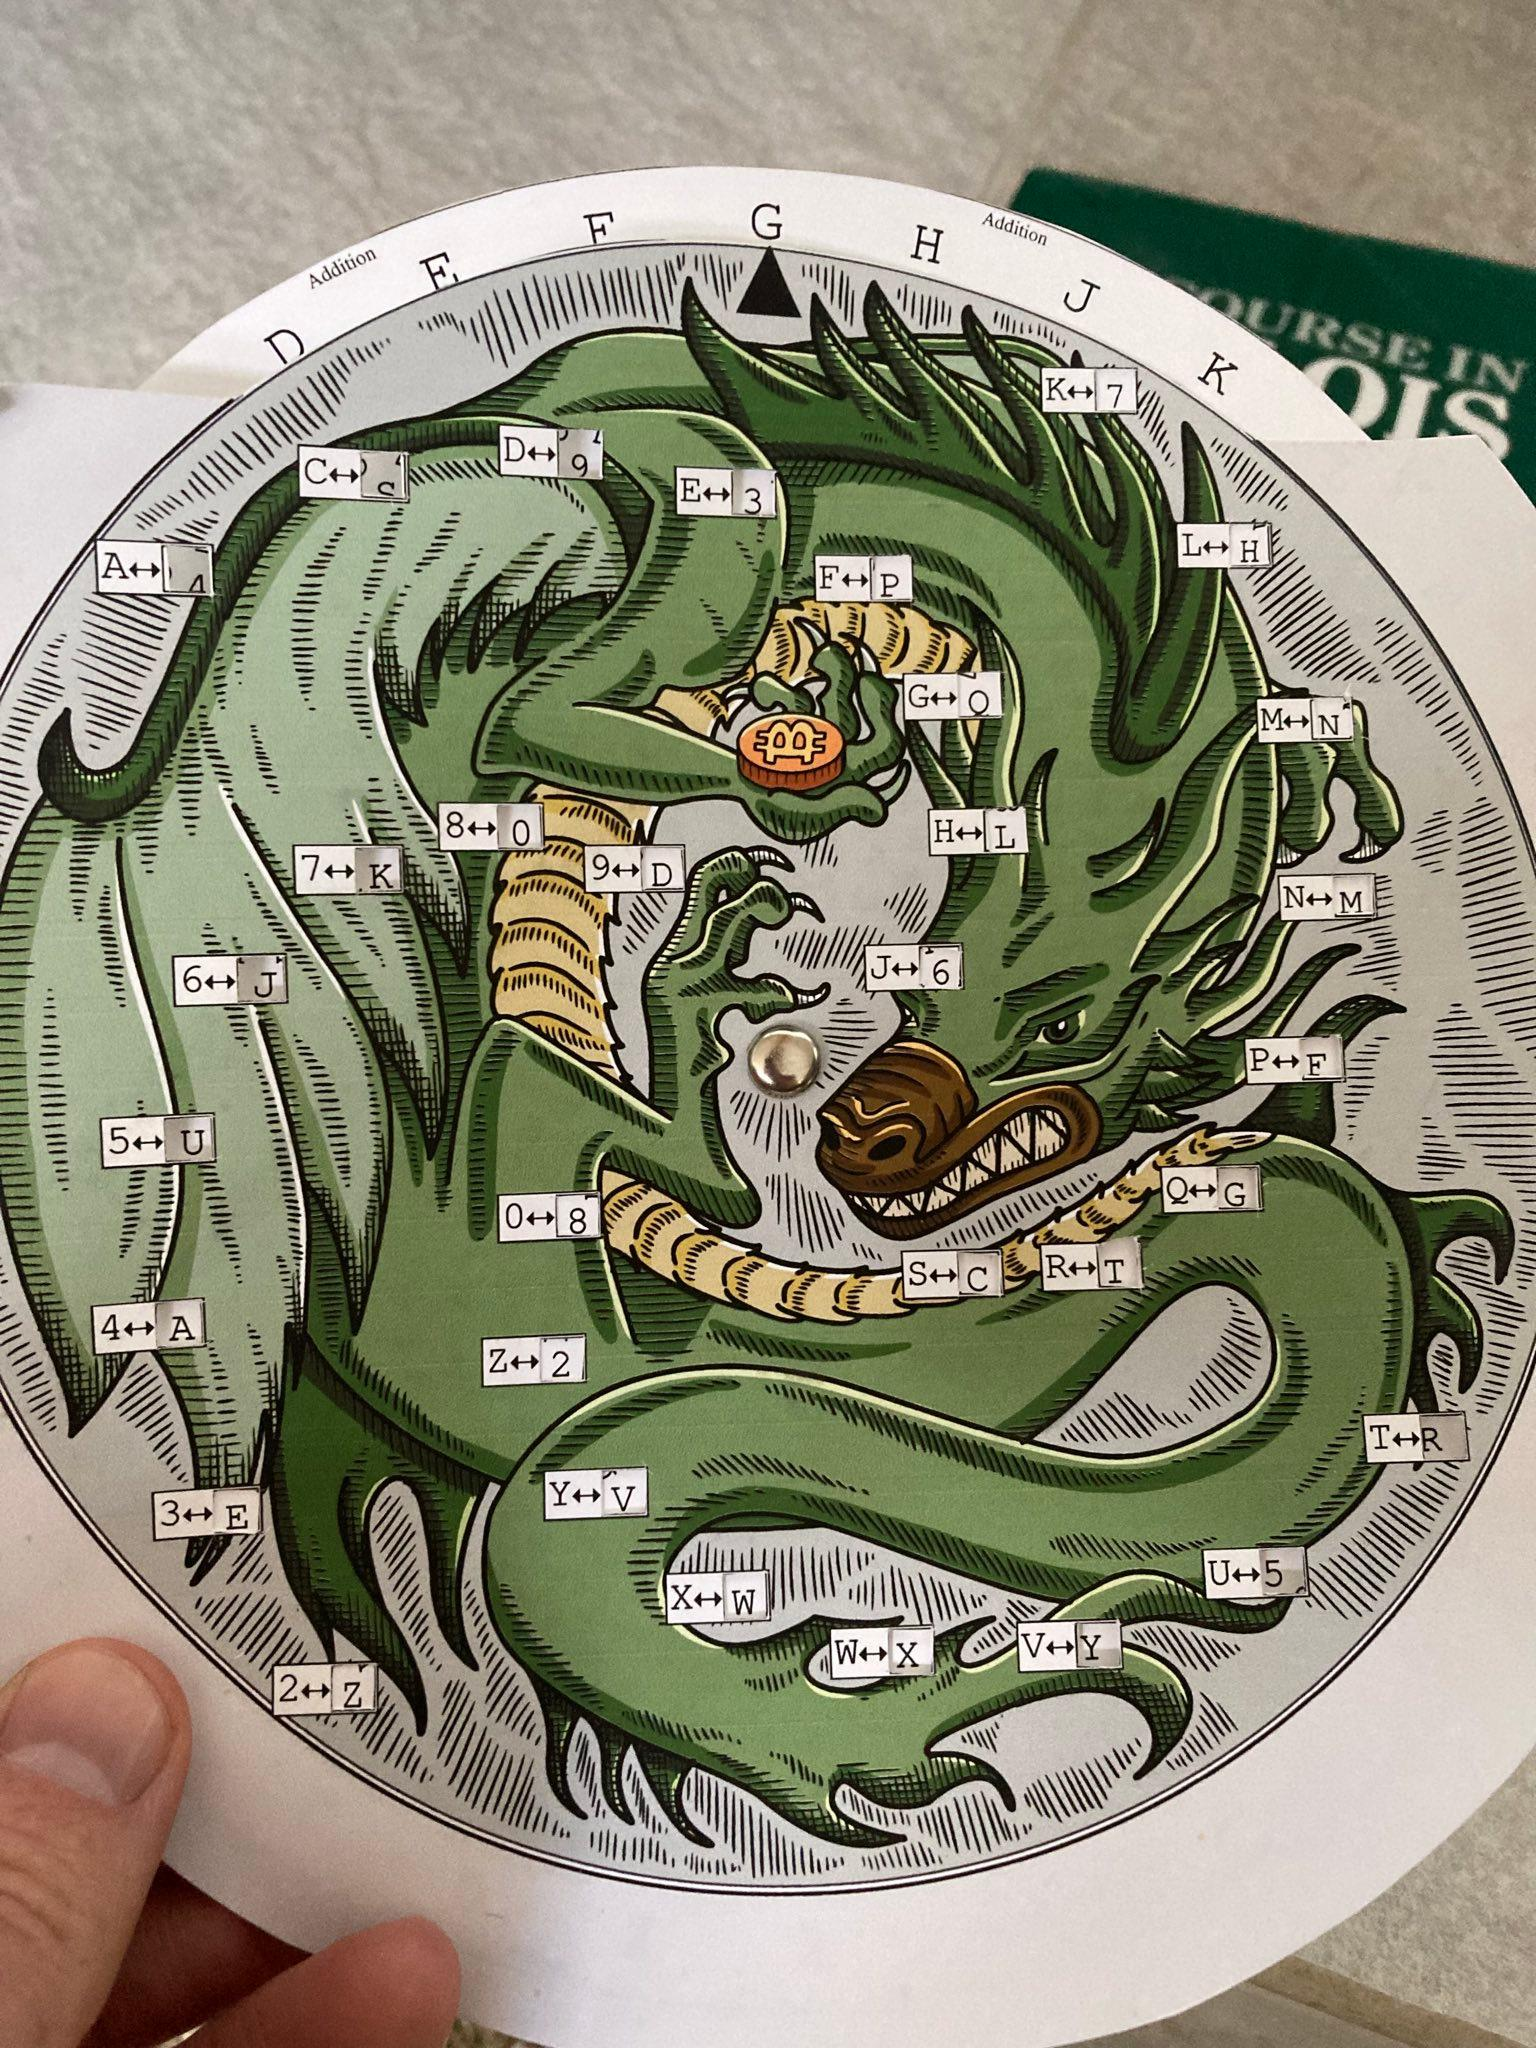
\includegraphics[scale=0.25]{images/addition-wheel.jpg}\end{center}


This volvelle computes addition in $\fttwo$. To compute $x+y$, rotate so that
the pointer is pointing at either $x$ or $y$, then look up the other one on
the front page. It is instructive to observe that the expected symmetries are
there: $x+y=y+x$, $x+x=Q$, $x+Q=x$, etc.

\paragraph{Volvelles and Algebraic Structure.} The addition wheel has 32 holes cut
in the face, corresponding to the 32 bech32 characters. If all 32 rotations
of the volvelle revealed distinct locations on the bottom wheel, it would
require 1024 symbols to be printed on the bottom wheel --- but if there
were algebraic structure relating the results of different volvelle positions,
we could reduce this number.

We will return to this idea in the next section, about slide rules, but for now
we simply observe that we did \textbf{not} reduce the number of symbols from
the maximum 1024.

Why not? Well, observe that the way to reduce symbols is to have two windows at
the same radius from the center of the volvelle. Then on the bottom sheet, a
single circle of values would provide the revealed symbols for both windows.
Let's say that one window is labeled $x\to$, and the other labeled $y\to$. Then
since the windows are at a fixed angle $\theta$ from each other (being printed
on the same solid sheet of paper), we would require the bottom circle of values
to satisify
\[ \textnormal{for all } z\in\fttwo:\qquad x + z \textnormal{ and } y+z \textnormal{ are at angle $\theta$ to each other} \]
Now, $x+z$ and $y+z$ differ by the fixed quantity $x+y$ (recall we are in
characteristic 2), so this can be restated as
\[ \textnormal{for all } z\in\fttwo:\qquad z \textnormal{ and } z+(x+y) \textnormal{ are at angle $\theta$ to each other} \]
Then observing that $(x+y) + (x+y) = 0$, two applications of the above equation
give us
\[ \textnormal{for all } z\in\fttwo:\qquad z \textnormal{ is at angle $2\theta$ from itself} \]
It is now clear that if we either need to repeat characters (defeating the goal
of reducing the amount of symbols on the bottom wheel) or have $\theta=180^\circ$.

Okay, so perhaps we can get a 50\% reduction in density for the bottom wheel, by
setting $\theta=180^\circ$ and having the windows on opposite sides of the top
wheel be at the same radius and use the same set of bottom-wheel symbols.

Let's play this out. Take, for example, the \vc{A} and \vc{T} windows on the
addition volvelle. These differ by \vc{K}, so we require that on the bottom
wheel, symbols at this radius differ from their opposite symbol by \vc{K}.
If the top wheel is pointing at some symbol $a$, and we turn it $180^\circ$
to $b$, we have simply exchanged the values in these windows, i.e.~added
\vc{K} to both. But this implies that $a+b=\vc{K}$.

In other words, for this compression to work, we need every pair of opposing
symbols to add to \vc{K}; i.e.~we need to take the sixteen 2-element cosets
obtained by modding out by \vc{K} and then order the symbols so that each
coset's members appear opposite each other.

It can be seen, by modding out by every possible symbol, and trying various
orderings of the resulting cosets, that no such choice will lead to a
``natural'' ordering\footnote{There are 16 cosets, so $15\approxeq2^{40}$
different arrangements around a circle. Then you can exchange the members
in each coset, for another $2^{15}$ possibilities. So an exhaustive search
would require about $2^{55}$ work. I did not do an exhaustive search, so I
may be wrong in claiming that ``no such choice'' works. But I spent several
hours starting from random permutations and then looking for local optima
and never got very close. My measure of ``naturalness'' was to take the
distance $d$ between each character and its alphanumeric successor, and to
sum all the $2^d$s.}. This means that to get this compression, we'd need
to reorder the wheel such that users wouldn't know which direction to spin
to find a desired symbol, and the resulting harm to usability would exceed
the benefit of having larger windows.

If this argument was too abstract, take the addition volvelle and spin it to
\vc{C} (one right of \vc{A}) and look at the symbols in the \vc{A} and \vc{T}
windows. Then spin it $180^\circ$ to \vc{U} (one right of \vc{T}) and look
at the same symbols. You will see different symbols. For this scheme to work,
they would need to be the same symbols. Ergo, we'd have to reorder the symbols
in a confusing order to make this work.

(By the way, this \emph{could} be made to work if we rearranged our mapping
between bech32 symbols and $\fttwo$ objects so that the \vc{K}-cosets, or
whatever, were naturally ordered. But deviating from the bech32 spec in this
way, for such a minor benefit in volvelle layout, doesn't seem worth the
potential confusion/incompatibility between the schemes.)

\subsection{The Fusion-Translation Wheel}

\paragraph{Fusion.}
While the addition volvelle could not be re-arranged to reduce the number of
symbols beyond 1024, let's consider the second operation we might like to do:
\emph{multiplication}.

For reasons that we will describe later, when multiplying in $\fttwo$ it turns
out that we want to use the alternate symbol alphabet rather than the bech32
alphabet. We also don't care so much about multiplication by zero, which always
results in zero, which we can tell the user rather than putting it into a
volvelle.

Now, we have 31 nonzero elements, so a volvelle would naively have $31^2=961$
entries. Can we do better? Using the same reasoning as with the addition volvelle,
if we wanted two windows $x\to$ and $y\to$ to share a radius, we'd need that
\[ \textnormal{for all } z\in\fttwo:\qquad xz \textnormal{ and } yz \textnormal{ are at angle $\theta$ to each other} \]
We have a group under multiplication with 31 elements in it. It is then a fact
that if we choose any element $\alpha\in\fttwo^*$ except 1, that $\alpha$
\textbf{generates} the group. Meaning that every element $z$, including 1,
can be written as $z=\alpha^{i_z}$ where $i_z$ is some integer modulo 31. So we
may write
\[ \textnormal{for all } \alpha^{i_z}\in\fttwo:\qquad \alpha^{i_x}\alpha^{i_z} = \alpha^{i_x+i_z} \textnormal{ and } \alpha^{i_y}\alpha^{i_z} = \alpha^{i_y+i_z} \textnormal{ are at angle $\theta$ to each other} \]

By squinting at this for a moment, you can observe that if $\theta$ is one 31th
of a full rotation, and we make sure that each $\alpha^i$ on the front wheel is
followed by $\alpha^{i+1}$, then \emph{every single window can have the same
radius}. In fact, we don't need windows, since the bottom wheel now has only a
single circle of symbols, all of which are always visible.

This is the intuition behind the \textbf{multiplication wheel}, which is actually
a \textbf{circular slide rule}:

\begin{center}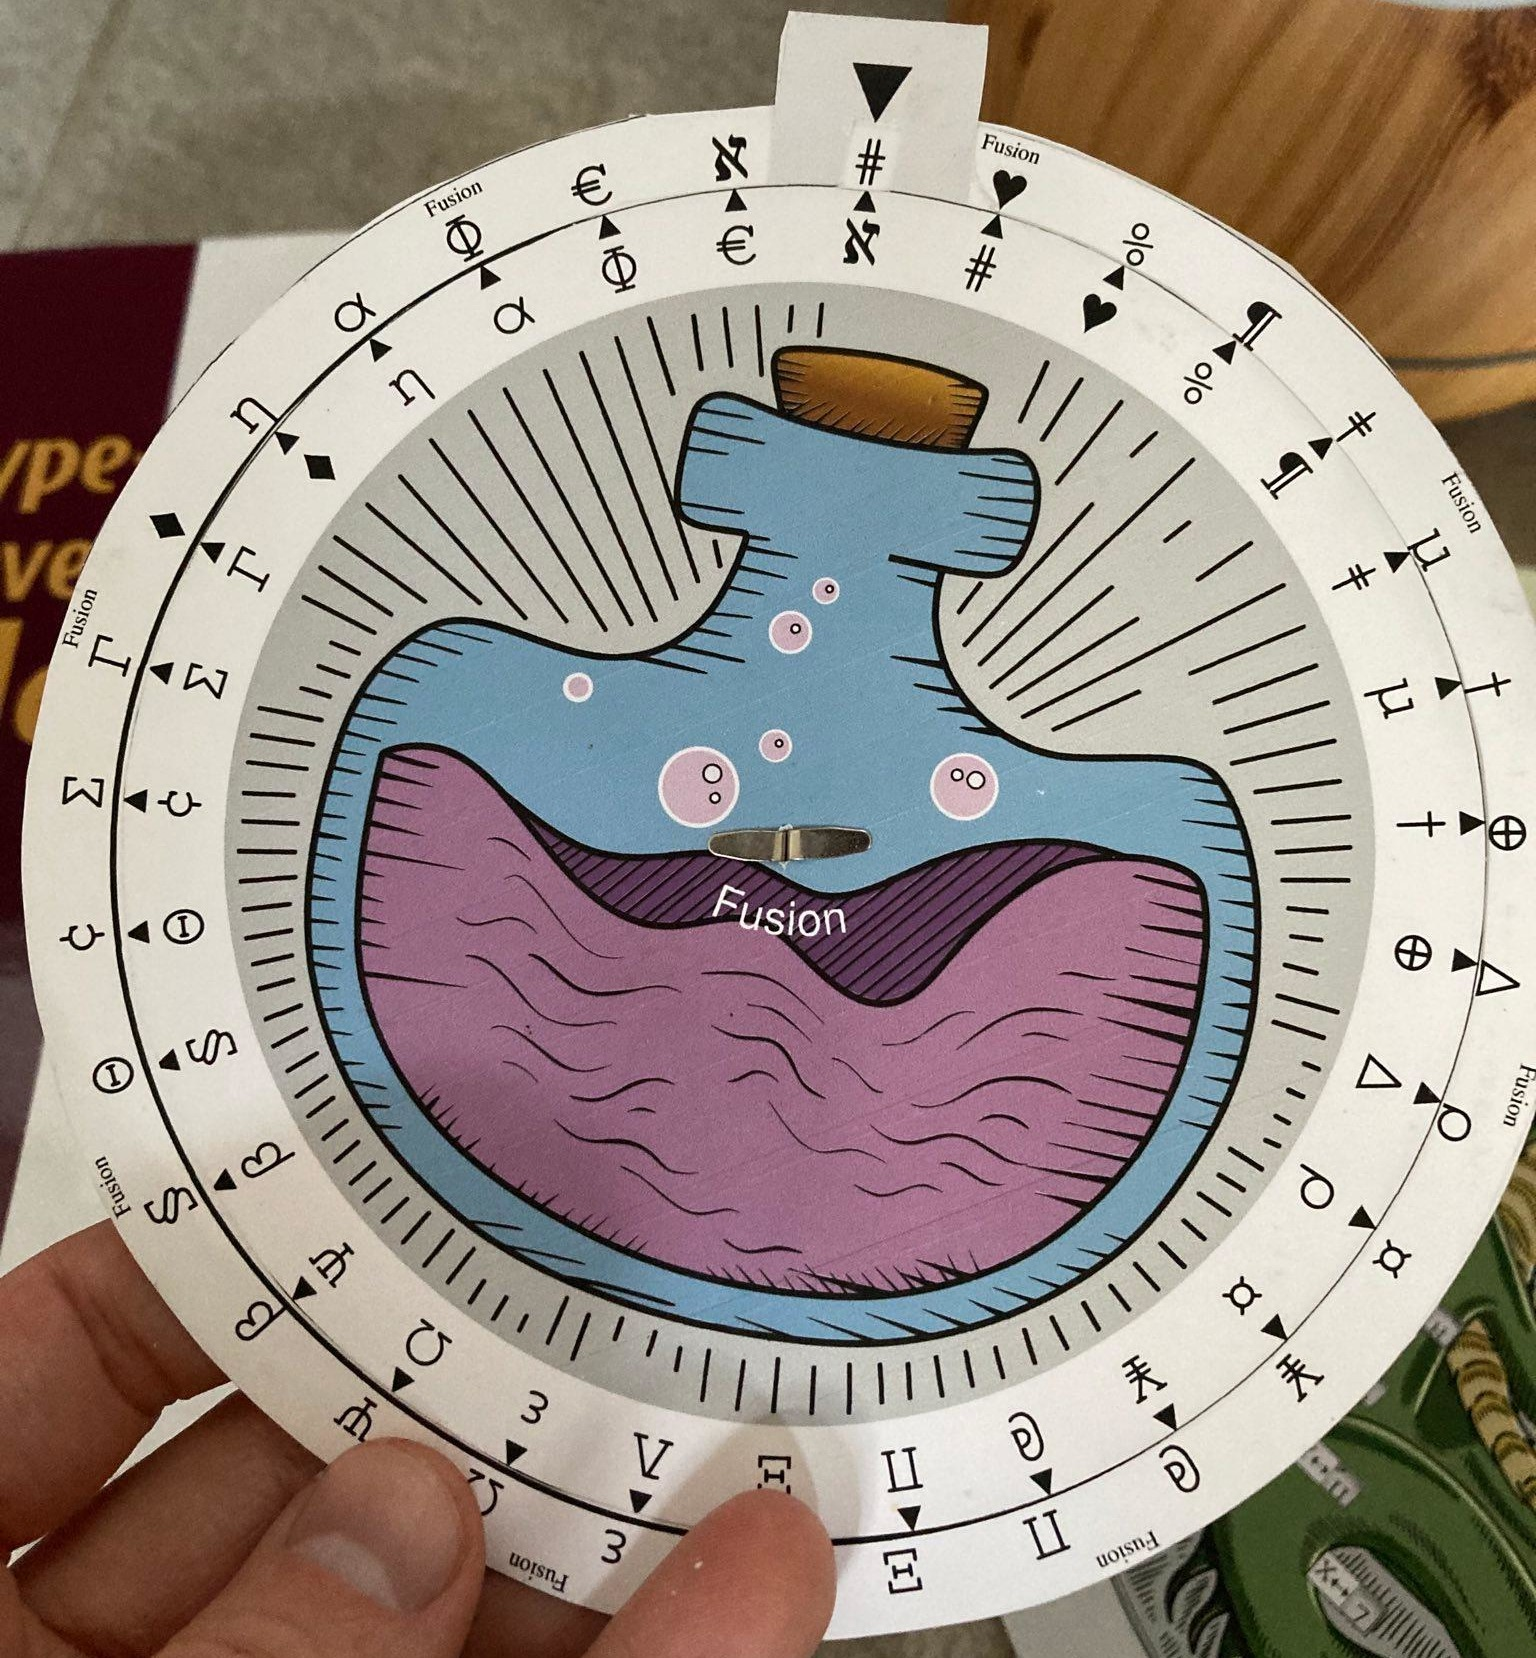
\includegraphics[scale=1.00]{images/fusion-wheel.jpg}\end{center}

We use the term \textbf{fusion} rather than \emph{multiplication} because we were
concerned that by having wheels labeled both ``addition'' and ``multiplication'',
that users may use their intuition about these operations on the integers, and
take incorrect shortcuts.

\paragraph{Translation.} There are actually two kinds of multiplication that
we might want to do: symbol-by-symbol multiplication and symbol-by-bech32-character
multiplication. The former we called fusion, and latter we refer to as
\textbf{translation}.

Algebraically, fusion and translation are identical, of course. But in
practice, fusion is used to multiply $k=2$ Lagrange basis polynomials
(encoded as symbols) to get $k>2$ basis polynomials (also symbols).
Meanwhile transalation is used to multiple the basis polynomials (symbols) by
share values (characters) to get translated shares (characters).

So by using different names for the wheels, and different encodings of the
underlying field elements, we have implemented a ``type system'' which makes
it hard for users to do operations in an incorrect order.

Since translation is identical to fusion, we might hope that we could
construct the translation slide rule by simply relabelling the fusion one.
Indeed, we could do this by changing the inner wheel to use bech32 characters
rather than symbols. Then to translate a character $c$ by a symbol $\sigma$,
for example, the user would turn the wheel to point to $c$, look for
$\sigma$, and find what it points to.

There are a couple minor issues with this approach:
\begin{itemize}
\item Because the correspondence between bech32 characters and $\fttwo$
does not have any algebraic structure, ordering alphanumeric characters by
increasing powers of $\alpha$ results in an unintuitive ordering.

We have chosen to just live with this problem. All the characters are visible
at the same time, so it isn't nearly as a bad a usability burden as it would've
been with a volvelle.
\item Since zero (\vc{Q}) is a valid share value, we actually do need to think
about multiplication by 0. This differs from the fusion case, since zero is not
a valid Lagrange basis polynomial. (0 can only be obtained by trying to use the
\vc{S} share as an \emph{input} rather than \emph{output}. But as we will see
in the next section, the Recovery Wheel won't let you do this.)

We solve this by just printing $\vc{Q}\leftrightarrow\vc{Q}$ on the handle of
the slide rule.
\end{itemize}

The biggest issue with just relabeling the inner wheel is that the user is
trying to map bech32 characters to bech32 characters, but indexing this mapping by
a symbol. So if she wants to translate a share by $\sigma$ say, for all 48
characters in her share, she'll need to rotate the wheel to the input
character then check where $\sigma$ points to find the output character.

This is tiring and error prone.
It would be better if she could just turn the wheel to $\sigma$ and then look
up every character without further rotations. How can we achieve this?

After several abortive attempts to add a third circle of characters to the
volvelle, Leon had the idea to put the Translation Wheel \emph{on the back of the
Fusion Wheel}. Then the user can use the Fusion side to index the mapping, then
flip over the wheel and use the Translation side to actually do the mapping!

Of course, we are mathematicians, so while we have brass fasteners, we have
no glue. So the actual assembly method is to print both sides attached to
each other, then fold them together. We then have two slide rules, whose
top and bottom wheels are now the ``outer'' and ``inner'' wheels, and which
are on opposite sides of the same pages.

\begin{center}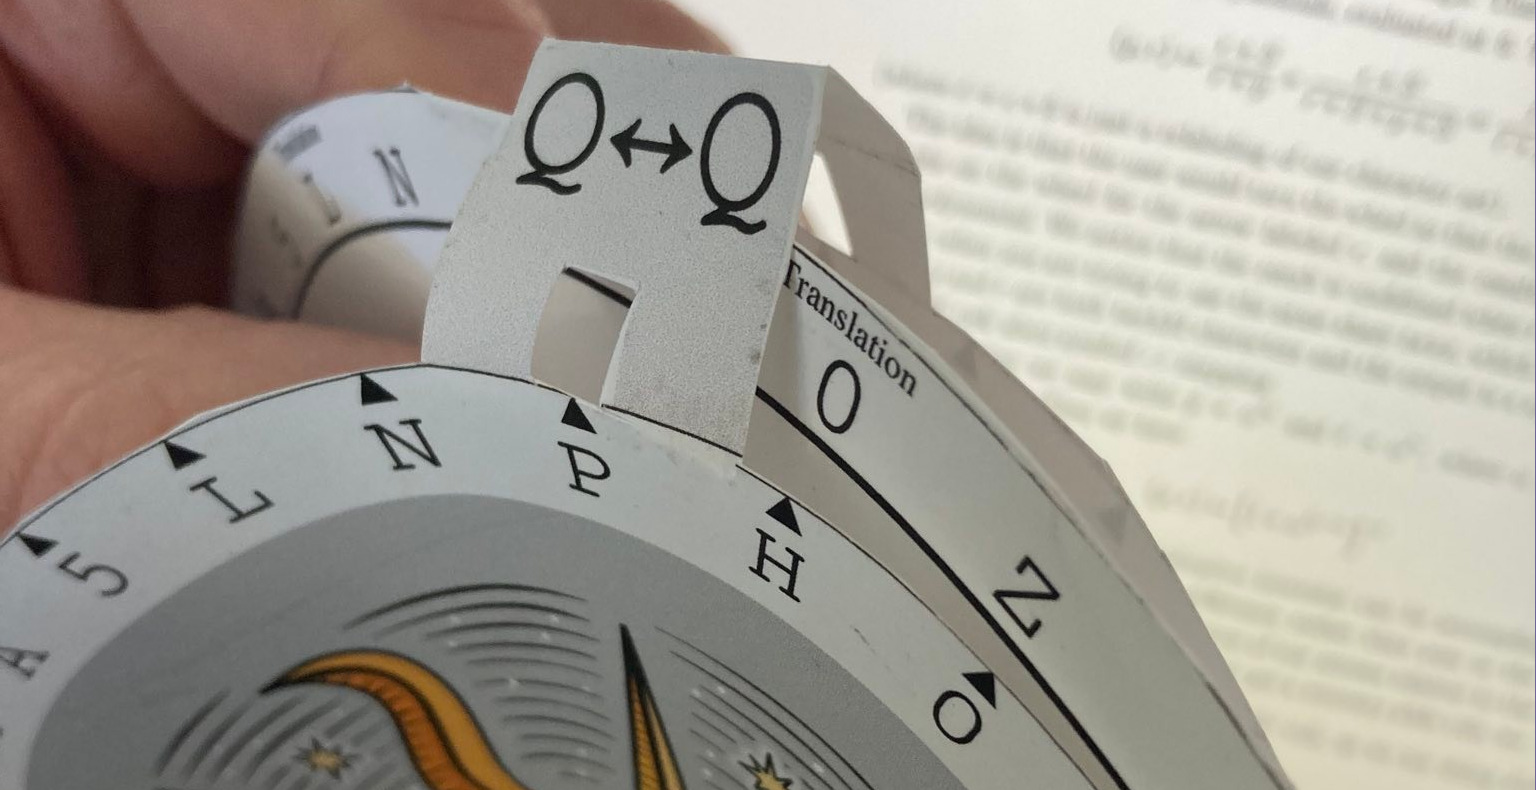
\includegraphics[scale=1.00]{images/fusion-fold.jpg}\end{center}
\begin{center}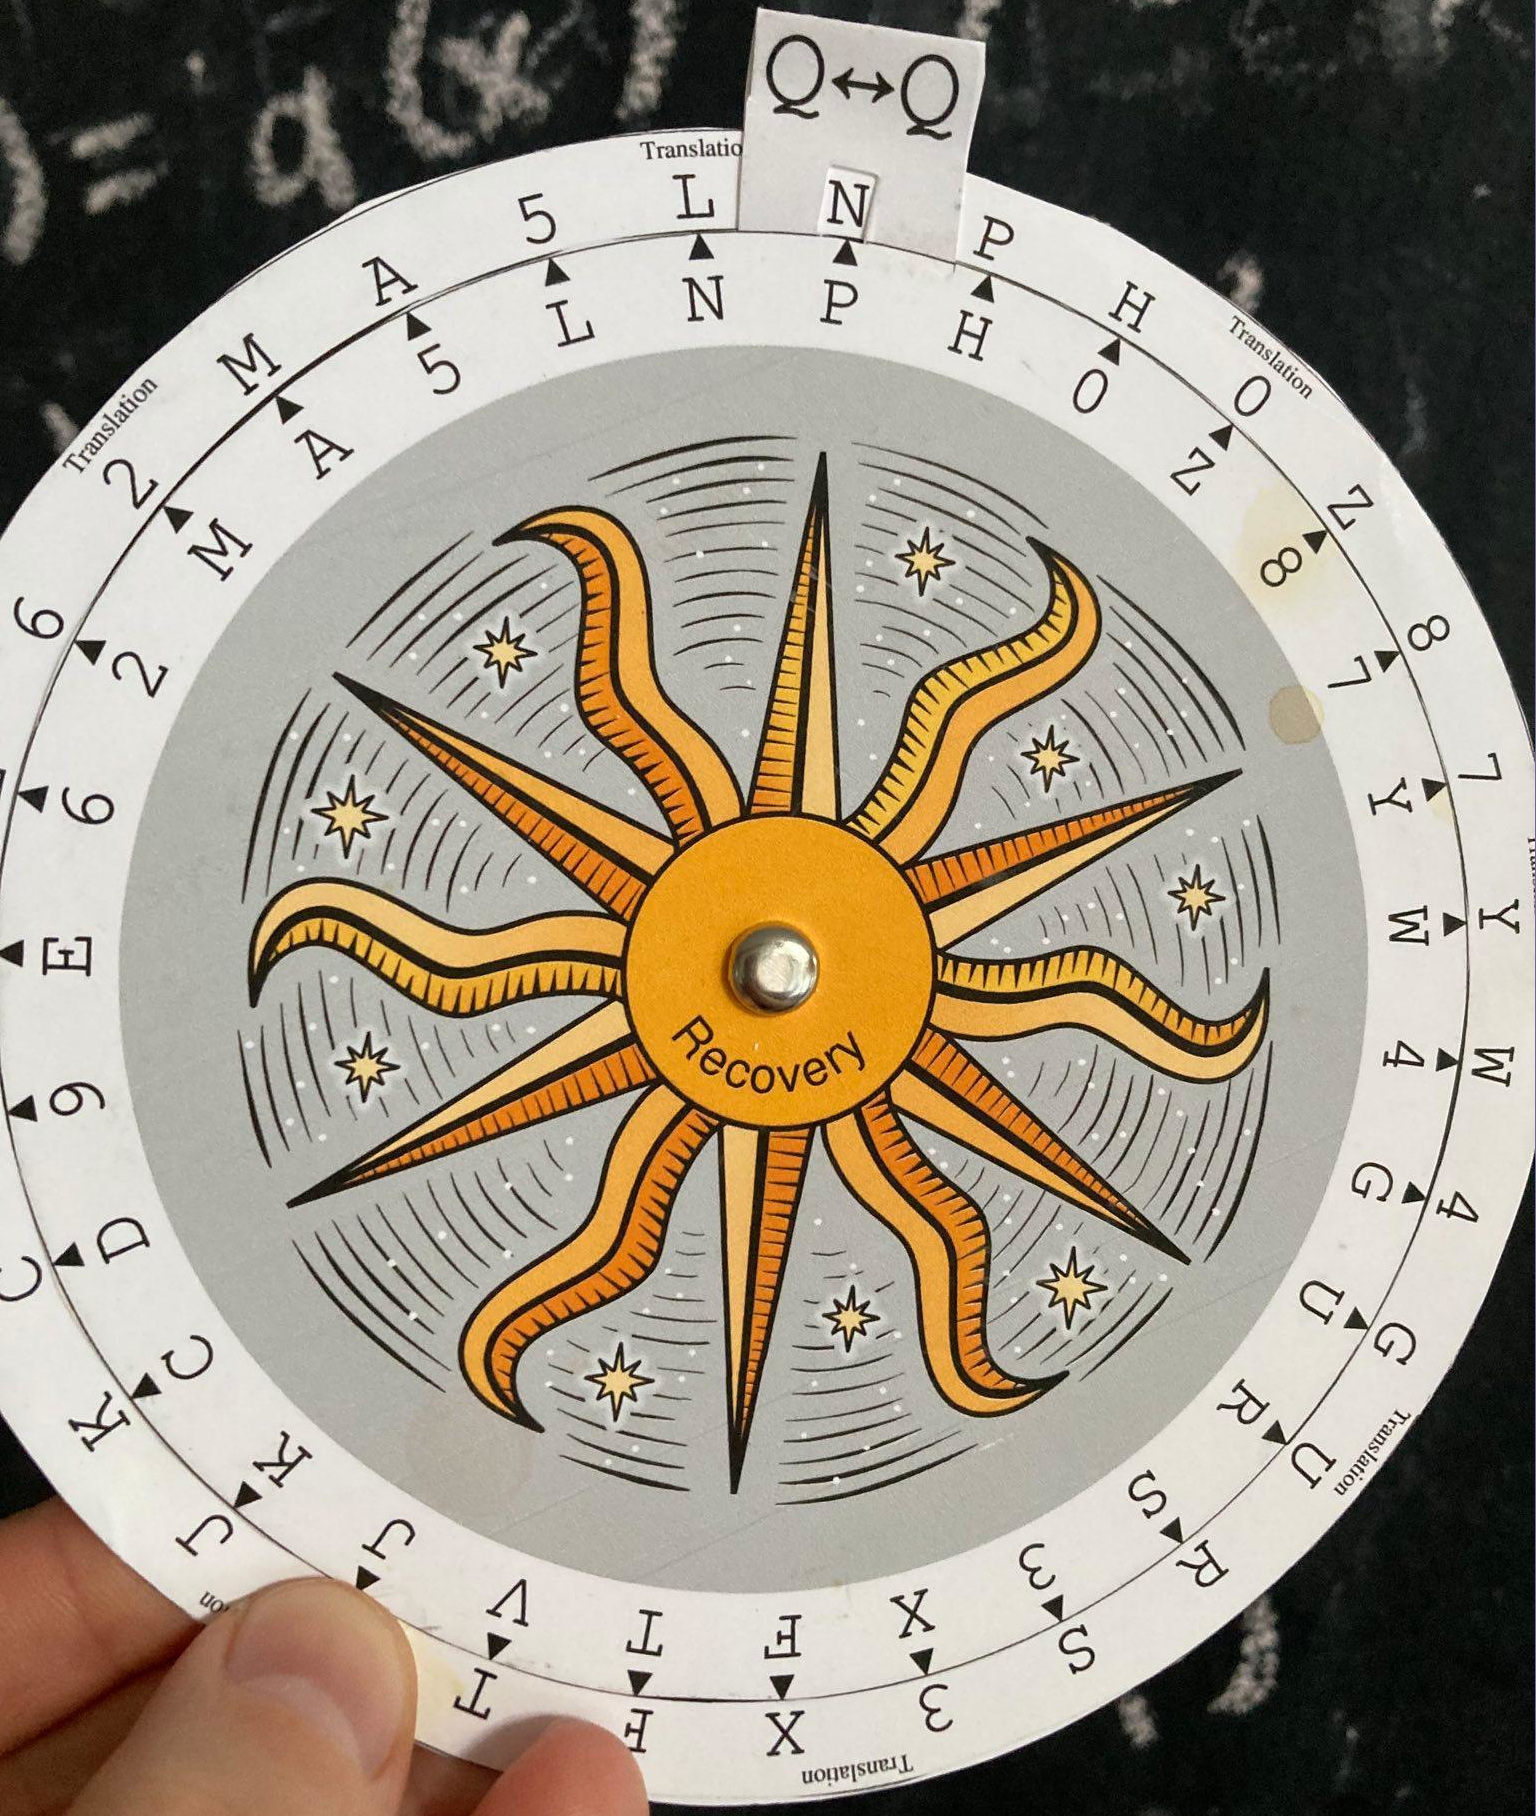
\includegraphics[scale=0.80]{images/translation-wheel.jpg}\end{center}

(The wheel in the photo is incorrectly labeled ``Recovery'', because I messed
up the PostScript and didn't notice before printing.)

\subsection{The Recovery Slide Rule}

There is one remaining paper computer to design. This one is the \textbf{Recovery
Wheel}, which computes Lagrange basis polynomials, evaluated at \vc{S}. That is,
it computes the map
\[ (p, r) \mapsto \frac{r + S}{r + p} = \frac{r + S}{r + S + p + S} \eqqcolon \frac{\hat{r}}{\hat{r}+\hat{p}} = \frac{1}{1 + \hat{p}/\hat{r}} \]
(where $\hat{c}\coloneqq c+\vc{S}$ is just a relabeling of our character set).

Note that both inputs are bech32-encoded share indices, while the output is
a symbol-encoded Lagrange basis polynomial evaluated at \vc{S}.

The idea is that the user would turn the wheel so that the pointer points at
share index $p$, looks on the wheel for the arrow labeled $r$, and the resulting
symbol is the Lagrange basis polynomial. We notice that the result is undefined
when $r = p$, which corresponds to the case when you are trying to use the same
share twice, which makes intuitive sense.

Now, as before we may write $\hat{p}=\alpha^{i_{\hat{p}}}$ and
$\hat{r}=\alpha^{i_{\hat{r}}}$, where $\alpha$ is a generator of our multiplicative
group. Then we have
\[ (p, r) \mapsto \left[ 1 + \alpha^{i_{\hat{p}} - i_{\hat{r}}} \right]^{-1} \]

The addition of 1 and the multiplicative inversion can be accomplished by more
relabeling, and the fact that we have a difference rather than sum in the exponent
of $\alpha$ can be accomodated by reversing the direction of our arrows relative
to the arrows on the multiplication wheel.

As with the Translation Wheel, we are indexing by a different set than either
our input or output. However, the Recovery Wheel only needs to be used once per
share, so it is fine for it to be a bit less convienent to use. The real usability
concern is that the use of bech32 characters for both indexing and output makes
it quite easy to accidentally use the wheel backward.

Putting it all together, to get a recovery slide rule, we
\begin{enumerate}
\item Reverse the arrows in our multiplication slide rule, as we are doing
division rather than multiplication.
\item Apply $x\mapsto x+\vc{S}$ to the inputs (which are now on the bottom
wheel).
\item Apply $x\mapsto[1+x]^{-1}$ to the output (on the top wheel).
\item Since 0 is not a possible output value, there is a blank space on the top
wheel, which conveniently is located directly below the handle. We can take
advantage of this blank space to label the handle ``share to translate'', which
hopefully will guide users to use the device correctly.
\end{enumerate}

\begin{center}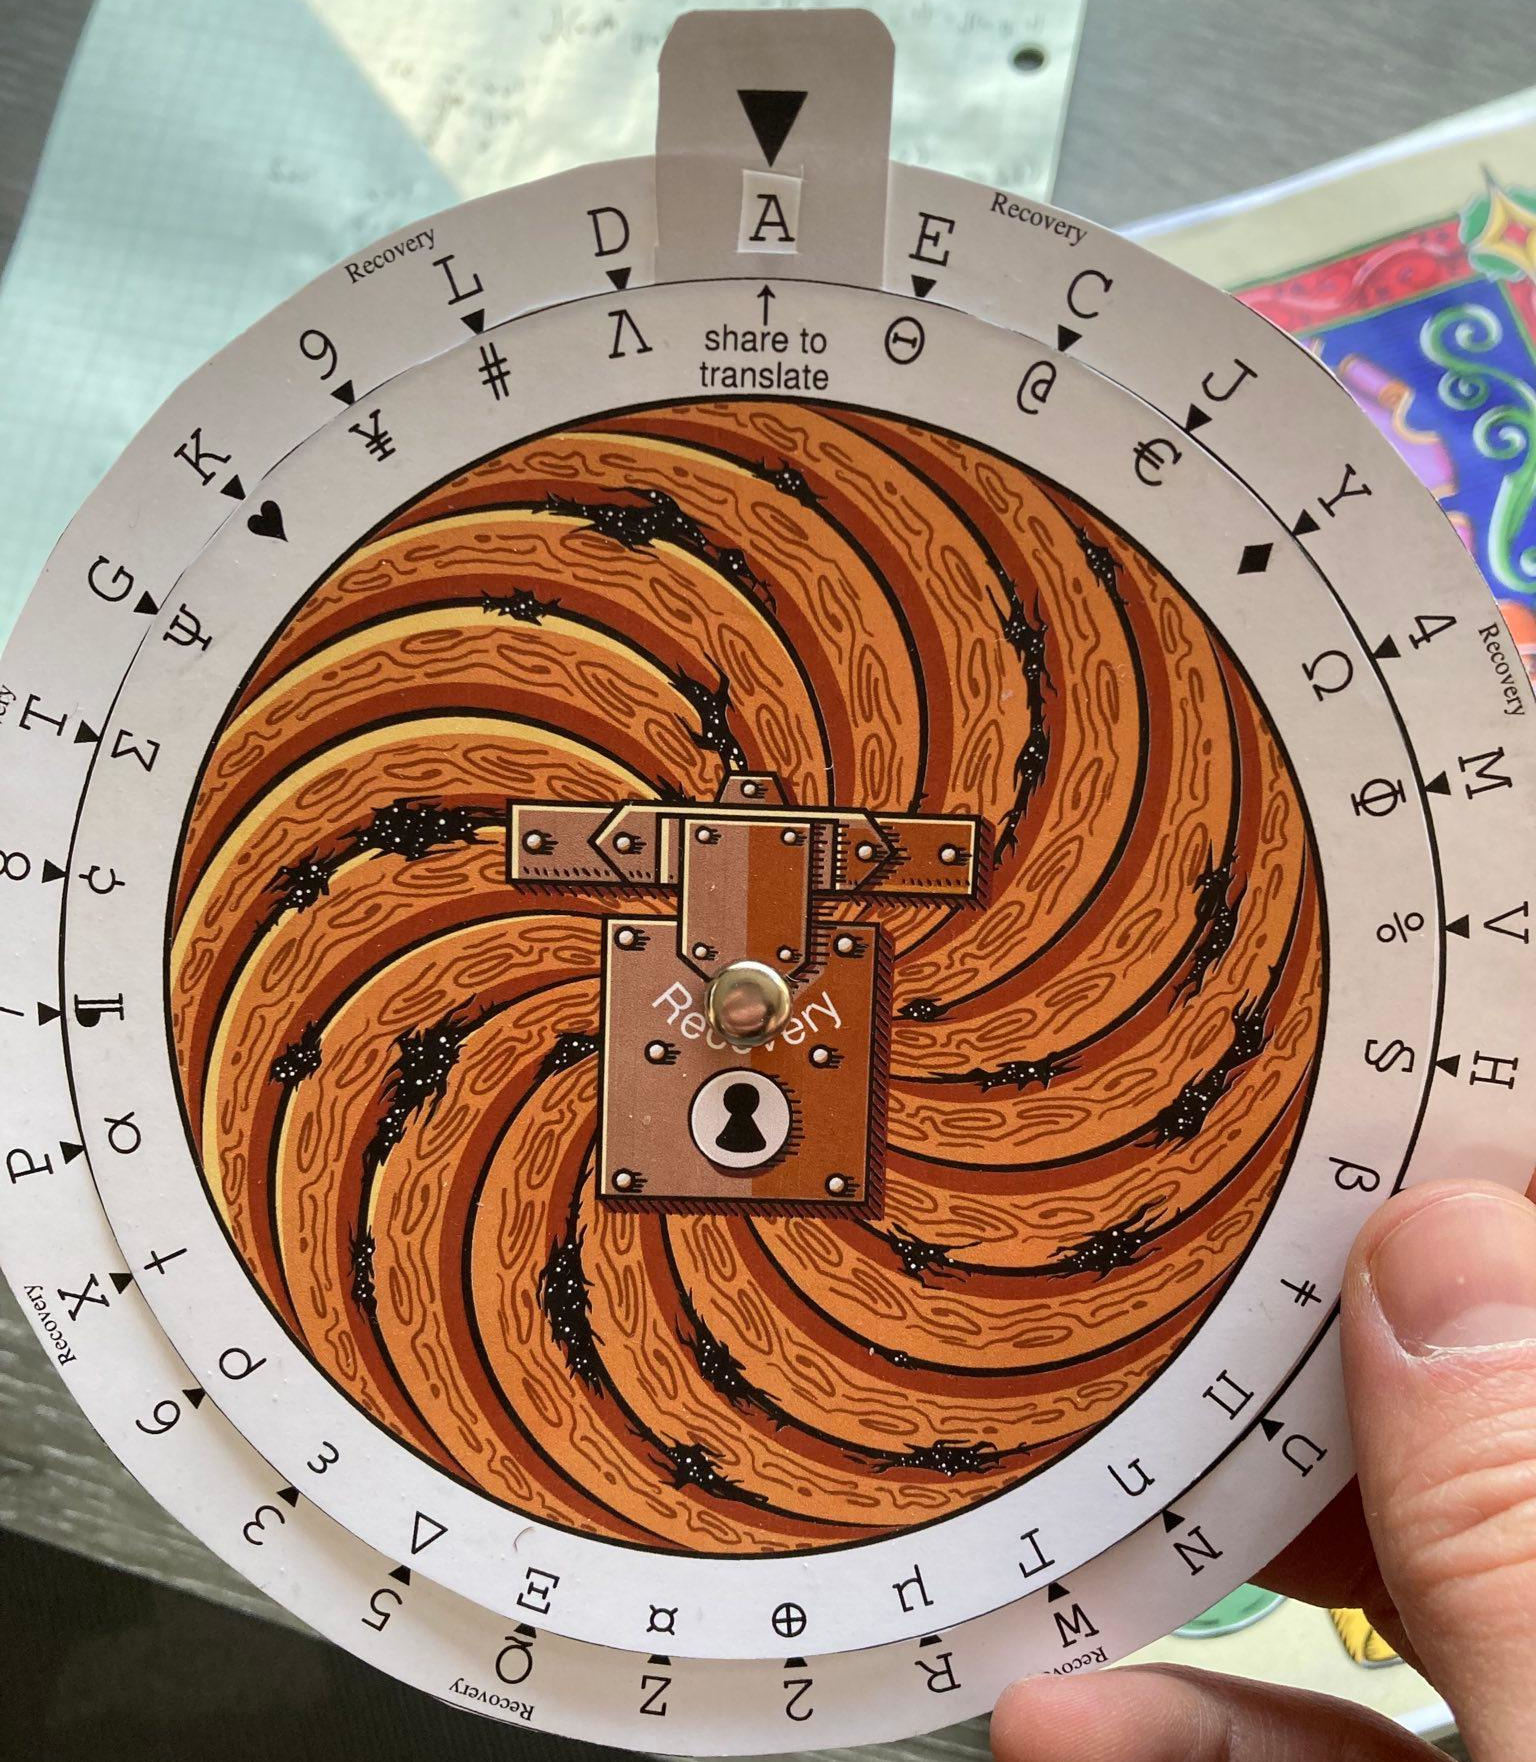
\includegraphics[scale=1.00]{images/recovery-wheel.jpg}\end{center}

Finally, we observe that, if we center our slide rule on the $\alpha^0$ output
slot (the one with the pointer on it, rather than a symbol), looking $j$ positions
to the left and right we have the values
\[ \left[ 1 + \alpha^{-j} \right]^{-1} \textnormal{ and } \left[ 1 + \alpha^j \right]^{-1}  \]
and it can be computed directly that these sum to 1.
In fact, this is exactly the relation between pairs of Lagrange basis polynomials
for the case $k=2$. (There are only two of them, and they add up to one because
Lagrange basis polynomials form affine sets.) So on the plain (non-art-covered)
version of this wheel, we can draw horizontal lines between these pairs, making
the wheel visually distinct from the other plain wheels and also guiding the user
in the $k=2$ case.\footnote{This was another innovation from Leon, who observed that
to look up the basis polynomials for $k=2$, you turn to one symbol and look up the
other; then swap the symbols and repeat. So by some sort of symmetry of turning, the
resulting outputs will be pairs of symbols opposite each other.

I'm not sure I see the symmetry he was referring to, but there is a simpler
algebraic reason: when you exchange $r$ and $p$, as you do when computing the
two Lagrange basis polynomials for the $k=2$ case, you replace $\hat{r}/\hat{p}$
with its reciprocal, which is the same as mirroring it over the $\alpha^0$
position on a slide rule. Then the fact that these add to 1 is just a restatement
of the fact that Lagrange basis polynomials form an affine set.}

\paragraph{The two alphabets.}
Now that we have all four of our paper computers defined, we can see the
justification for having two alphabets: \emph{share data} and \emph{share
indices}, which are secret and need to be stored, are represented by bech32
characters, while \emph{Lagrange multipliers}, which are not secret and
never stored, are represented by symbols.

Because share indices are actually encoded as share data, these arguably-distinct
kinds of data must be encoded the same way. There does not seem to be any ergonimic
way to avoid this.

This user-centric categorization is conveniently reflected in the operations that
need to be done:

\begin{itemize}
\item Share data may be added to other share data, but it is never multiplied
by other share data, only by Lagrange basis polynomials (i.e.~``translation'').
\item Lagrange polynomials never added to each other, only multiplied by
each other (i.e.~``fusion'') or by share data (i.e.~``translation''). In these
two cases the output data is different.
\item To do share derivation or recovery, a user cannot even start without
obtaining a Lagrange multiplier, which will come either from the Recovery Wheel
or from tables provided in the booklet. This ensures the user has obtained all
the necessary data before being able to start secret sharing.
\end{itemize}

More explicitly, both share creation and secret recovery are implemented as
Lagrange interpolation using Equation~\eqref{eq:linterp} on page~\pageref{eq:linterp}.
In that equation, we are performing a linear combination of $y_i$ values, which
are share data (bech32 characters), multiplied by evaluated Lagrange basis
polynomials $\ell_i(x)$s (symbols).

The Lagrange basis polynomials are always products of the form $(x + y)/(x + z)$.
The Recovery Wheel and Fusion Wheel allow the user to compute these products when
they are evaluated at \vc{S}, regardless of which of the combinatorially-many sets
of shares they may have started with. During share derivation, the complete products
are pre-computed and provided in tables, and require the user to begin with a
prescribed set of initial shares.

\section{BCH Codes}

Now we have our mathematical foundation, from field arithmetic to Lagrange
interpolation, and have seen how to express this in volvelles. The final
component of our scheme is the checksum, which is a \textbf{BCH code}. There is a
rich and enormous theory underlying BCH codes, and linear codes in general,
but we will take an operationalist point of view and summarize just the facts
that we need:

An \textbf{error-correcting code} is a mapping from a set of raw data, called
\textbf{messages} into a larger set of \textbf{codewords} which have
some extra algebraic structure. In particular, between every pair of
codewords there is a minimum \textbf{distance} $d$, which measures the
number of characters at which the two codewords differ.

Since all codewords differ by at least the minimum distance $d$, if there
are at most $d-1$ errors in a codeword, the result is guaranteed not to
be a valid codeword, and to be detected as an error pattern. If there are fewer
than $d/2$ errors, the correct codeword is uniquely determined by being
the closest codeword to the error pattern, which means that this many
errors can, in principle, be corrected.

A \textbf{BCH code} is a specific type of error-correcting code. In a BCH
code, codewords are constructed by encoding data as the coefficients of a
large polynomial, then affixing some number of \textbf{checksum characters}.
The checksum characters are chosen so that the full result is in
a specific residue class modulo a \textbf{generator polynomial} $G(x)$.

Given a potential codeword, there is a unique minimum-degree polynomial
equivalent to this codeword modulo $G(x)$, which can be found by modular
reduction. We refer to this reduced polynomial as the \textbf{residue}
of the codeword.

There are several properties of a BCH code that we will need:
\begin{itemize}
\item The \textbf{degree} of the code is the maximum degree of the roots of
its generator polynomial. (Since the generator polynomial is not, in general,
irreducible, this is \emph{not} the degree of the generator polynomial.)

The degree of our BCH codes, and that of bech32, is 2. Degree-1 BCH codes are
called \textbf{Reed-Solomon codes}.

The degree indicates the dimension of the extension field you need to work
in to do error correction. So for our codes, you would need to work in a
quadratic extension of $\fttwo$, i.e.~$\ftttwo$.

\item The \textbf{length} of the code is how long a coded message can be
(including the checksum!) for the code to retain its error-correcting
properties.

The length $\ell$ can be computed as the smallest polynomial of the form
$x^\ell - x$ that the generator divides. This can be seen by observing
that if you have a message of this length, that the $\ell$th character
will be interpreted as the coefficient of $x^{\ell-1} \equiv 1$ mod $G(x)$,
meaning that it will just mask your first character rather than being
checksummed independently.

We have two codes -- the ``normal'' codex32 has a length of 93. For 512-bit
seeds, we need more than 93 characters, so we use an alternate code of
length 1023. The length of bech32 is also 1023 --- although through
an exhaustive search, it was found to have better error detection properties
than the algebra would suggest, up to length 71.

\item The $m$-value, or \textbf{target residue}, is the specific residue that
all codewords must must have modulo $G$. All $m$ values are equivalent, in
the sense that it is easy to convert from one $m$ value to another (simply
add the difference to the checksum characters of every codeword).

But $m=0$ has the particularly bad property that any codeword can be extended
by addition of an arbitrary number of 0s to get another valid codeword. (This
highlights the fact that BCH codes are designed to handle only \emph{substitution}
or \emph{erasure} errors, not insertions or deletions.) Other small values of
$m$ have similar issues; bech32 was originally defined to have $m=1$ but later
needed to be modified to bech32m for this reason. bech32m uses a large $m$
instead\footnote{For more details, see
\url{https://gist.github.com/sipa/14c248c288c3880a3b191f978a34508e}}.

On the other hand, $m=0$ makes a BCH code a \textbf{linear code}, and brings
with it a ton of algebraic properties which are needed for analysis, so this
is what is used in the literature.

In practice it is common to use a string of all-bits-one for $m$. For our code,
we chose characters which spell out \vc{SECRETSHARE32} for the standard code,
and \vc{SECRETSHARE32EX} for the alternate one.

\item The \textbf{checksum length} is the number of extra characters that
need to be added to a string to ensure that it has the correct residue.
This value \emph{is} the degree of the generator polynomial.

Our standard code, of length 93, has a checksum length of 13. The alternate
code has a checksum length of 15.
\end{itemize}

We will return to BCH codes in the next section, when we discuss the Checksum
Worksheet and the properties of BCH codes which make them compatible with
Shamir's Secret Sharing.

\subsection{The \texttt{codex32} Checksum}

We now get into the meat of the document, where we descibe how the actual
user processes are implemented. We start with the checksum.

Our primary checksum is defined by a BCH code with generator polynomial
\begin{align*}
    G(x) = x^{13}
      &+ \vc{E}x^{12} + \vc{M}x^{11} + \vc{3}x^{10} + \vc{G}x^9 + \vc{Q}x^8 + \vc{E}x^7 \\
      &+ \vc{E}x^6 + \vc{E}x^5 + \vc{L}x^4 + \vc{M}x^3 + \vc{C}x^2 + \vc{S}x + \vc{S}
\end{align*}
Our alternate checksum has generator polynomial
\begin{align*}
    \hat{G}(x) = x^{15}
        &+ \vc{0}x^{14} + \vc{2}x^{13} + \vc{E}x^{12} + \vc{6}x^{11} + \vc{F}x^{10} + \vc{E}x^9 \\
        &+ \vc{4}x^8 + \vc{X}x^7 + \vc{H}x^6 + \vc{4}x^5 + \vc{X}x^4 + \vc{9}x^3 \\
        &+ \vc{K}x^2 + \vc{Y}x^1 + \vc{H}
\end{align*}
Because the alternate code has substantially the same properties as the primary
one, and the primary one is easier to work with, we will only focus on the
primary one from here on.

To interpret the $\fttwo$ elements such as $\vc{E}$, $\vc{M}$, etc., recall that
there is a table on page~\pageref{pg:f32table} containing all the elements and
their alternate encodings.

To checksum a string of bech32 characters $\{v_i\}_{i=1}^n$, we want to encode it
as a polynomial
\[ p(x) = x^n + \sum_{i=0}^{n-1} v^{n-i} x^i \]
such that $p(x)$ mod $G(x)$ is equal to \vc{SECRETSHARE32}, i.e.
\begin{align*}
\vc{S}x^{12} + \vc{E}x^{11} + \vc{C}x^{10} + \vc{R}x^9 + \vc{E}x^8 + \vc{T}x^7
    + \vc{S}x^6 + \vc{H}x^5 + \vc{A}x^4 + \vc{R}x^3 + \vc{E}x^2 + \vc{3}x + \vc{2}.
\end{align*}

Remembering throughout that an $n$-degree polynomial has $(n+1)$ terms, the way that
we achieve this for an arbitrary message $\{ v_i \}$ is to concatenate the target
residue \vc{SECRETSHARE32} to $\{ v_i \}$ as
\begin{equation}
 \hat{p}(x) = x^{n+13} + \sum_{i=0}^{n+13-1} v^{n+13-i} x^{i} \textnormal{ mod } G(x)
 \label{eq:modg}
\end{equation}
We call the thirteen resulting characters the \textbf{checksum} and replace our
copy of \vc{SECRETSHARE32} with them.

Why does this work? Basically, to get our residue to match some specific target, we
just need to subtract the existing residue from our string, then add the target. Since
both the existing residue and the target value have degree 12, this will affect only
the rightmost 13 charactes of our string.

So we multiply by $x^{13}$, moving our actual data to the left 13 spaces, and add
\vc{SECRETSHARE32}. Then the above instructions ``subtract the existing residue from
our string, then add the target'' are easy. First we add the target, which since we
are in characteristic 2, means zeroing out the \vc{SECRETSHARE32} we just added by
adding another one. Then we subtract the existing residue from this 0, which (again
because of characteristic 2, where negation is a no-op) means just copying it into place.

\subsection{The Checksum Worksheet}

As described in the last section, our checksum verification algorithm is: encode the
message as a polynomial, take it mod $G(x)$, and compare it against the fixed string
\vc{SECRETSHARE32}. The checksum generation algorithm is essentially the same:
append \vc{SECRETSHARE32} in place of the checksum, take the resulting polynomial
mod $G(x)$, then use the result as the actual checksum.

How do we do this in practice? In short, we build up our polynomial two characters
as a time: multiply by $x^2$, add two new characters, reduce, repeat. In detail:

\paragraph{Checksum Verification.}

\begin{enumerate}
\item Take the prefix \vc{ms1} and encode it as a bech32 human readable part (HRP),
which works out to \vc{RRQDN} (the process is to take the high 3 bits of each
8-bit ASCII character, followed by 0, followed by the low 5 bits of each character).
Prefix a 1, or \vc{P} in bech32. The resulting initial polynomial is \vc{PRRQDN}, or
\[ x^5 + \vc{R}x^4 + \vc{R}x^3 + \vc{D}x + \vc{N} \]
Multiply this by $x^{13}$ and reduce it mod $G(x)$. The result will be
\vc{33XW87RRYLJG}. This string is initially filled in in the checksum
worksheet.

\item Fill in the first 13 characters of the data to be checksummed. Add this to
the pre-filled values. The result will be the residue of \vc{ms1<first 13 user characters>},
and this is what the first three lines of the checksum worksheet compute.

\item Multiply by $x^2$ and fill in the next two characters of data. The multiplication
is done by shifting the characters two spaces to the left, equivalently, shifting the
entire rest of the worksheet 2 spaces to the right. This accounts for the diagonal
shape of the worksheet.

The resulting 3rd row has 15 characters, where the leftmost characters $\ell_1$
and $\ell_2$ are the coefficients of $x^{13}$ and $x^{14}$.

\item Reduce the whole string mod $G(x)$: first, compute the reduction of the
leftmost characters, $\ell_1x^{14} + \ell_2x^{13}$. This is a nontrivial
computation, so we simply provide a giant ``Checksum Table'' in which the user
can look up $\ell_1$ and $\ell_2$.

Copy the table entry into line 4. Then add the remaining 13 characters, which
are unaffected by reduction since $G$ has degree 13, to this.

It may be instructive to read the PostScript code for the Checksum Table, which
enumerates all the two-character possibilities, and for each one, computes
the reduction mod $G$.

\item Repeat the previous two steps: add the next two characters of data to the
right of the just-filled-in line, lookup the leftmost two characters in the
Checksum Table to fill in the next line, and add the results.

Repeat until you run out of data.
\item Check that the final result is \vc{SECRETSHARE32}.
\end{enumerate}

\paragraph{Checksum Generation.} This is basically identical to checksum verification,
except that the final 13 characters are initially not available. On the worksheet these
are colored pink to indicate to the user that she should stop filling random data into
the cells.

In the mathematical description we suggest concatenating \vc{SECRETSHARE} to the data
itself, then replacing it. It is equivalent to instead write \vc{SECRETSHARE} in the
in the bottom-most row (whose cells lie below the final 13 data cells), and then
``backsolve'' by subtracting (i.e.~adding) all the rows above it. This will place
the residue, our desired checksum, in the correct place.

\section{Secret Sharing}

In the Mathematical Preliminaries section we described Lagrange interpolation and
Shamir's Secret Sharing Scheme (SSSS). We defined the Fundamental Theorem of Computing
SSSS With Volvelles as the observation that Lagrange interpolation allows evaluating
a polynomial at a fixed point as an affine combination of its evaluations at other
fixed points.

As a consequence, any linear or affine relationship between the original evalutations
will be preserved. We will come to this in a moment, but first let's describe the SSSS
process.

\subsection{Computing SSSS}

There are two places where we use Lagrange interpolation:
\begin{itemize}
\item When creating a share with index $x$, we start with $k$ initial shares $x_1$,
$x_2$, \ldots, $x_k$ whose indices are always the first $k$ symbols of the bech32
alphabet \vc{A}, \vc{C}, \vc{D}, etc.

(There is an alternate process where the user starts with a fixed secret, in which
case $x_1$ is \vc{S} and the other $x_i$'s are shifted, but the rest is exactly
the same.)
\item When recovering a secret, we start with $k$ shares with indices $\{x_i\}_{i=1}^k$
which are fixed during recovery but unpredictable in advance, and compute the
\vc{S} share.
\end{itemize}

In both cases, the computation is straightforward: evaluate~\eqref{eq:linterp} as
\[ p(x) = \sum_{i=1}^k \ell_i(x) y_i \]
Here $y_i$ is the data of the $i$th share and $\ell_i(x)$ is a Lagrange multiplier
which must be computed by the user. We refer to these multiplies as ``Recovery
Symbols'' in the text. To avoid confusion, they are always encoded using the symbol
alphabet rather than bech32. The process for obtaining these is:

\begin{itemize}
\item During share creation, the evaluation points $\{x_i\}$, which are the
user's initial share indices, are always fixed. Therefore $\ell_i(x)$ is purely
a function of $x$ (the index of the share to be created) and $k$. There aren't
that many possibilities so we simply provide tables on the ``Constructing Shares''
page.

(It is instructive to modify the PostScript source for these tables to allow
``deriving'' the initial shares from themselves. You will find that the index for the initial
share under question becomes 1 ($\aleph$) while the index for all the other shares
is 0 ($\times$).)

\item During recovery, there are up to 31 outstanding non-\vc{S} shares and
the user has an arbitrary subset of $k$ of them. There are $\binom{31}k$
possibilities, which for $k=2$ is a reasonable number --- 465 --- but for
$k\geq3$ quickly grows out of hand, to 4495, then 31465, and beyond.

For $k = 2$ we provide a table, both in tabular form and in the form of a volvelle.
This is what the Recovery Wheel ultimately is, and at position $p$, window $w$ it
computes
\[ \ell_i(\vc{S}) = \frac{w + \vc{S}}{w + p} \]
Here position $p$ is the index of share $y_i$ whose multiplier is being computed,
and $w$ is the index of the other share. To avoid getting $p$ and $w$ confused,
we have written ``Share to Translate'' on the handle of the disc.

For $k \geq 3$, for target share $p$ (index of $y_i$) with other shares
$\{w_i\}_{i=1}^{k-1}$, we need to compute
\[ \ell_i(\vc{S}) = \prod_{i=1}^{k-1} \frac{w_i + \vc{S}}{w_i + p} \]
with notation chosen to highlight that \emph{the Lagrange basis polynomials for
$k\geq3$ are products of the basis polynomials for $k=2$}.

This fortuitous fact means that the user can compute polynomials $\ell_i(\vc{S})$
by looking up factors using the Recovery Wheel (rotate it to index $p$ then
read all the $w_i$'s off the front), and then multiplying all the results using
the Fusion Wheel. (Turn the wheel so it points to the first symbol, then look up
the second. Turn it to whatever the second symbol is pointing to, look up the
third, and so on.)

The Fusion Wheel is the only one which takes two symbols as input, and multiplication
is commutative so the order of inputs doesn't matter, so it is hard for the user
to do the wrong thing here.
\end{itemize}

Once the user has obtained the $\ell_i(x)$'s, the rest is simple: multiply each
cell of $y_i$ (the value of the $i$th share, encoded in the bech32 alphabet) by
$\ell_i(x)$ (computed above, encoded in the symbol alphabet) using the Translation
Wheel.

Again, the choice of alphabets and commutativity of multiplication make it hard
for the user to do the wrong thing.

This will give the user $k$ translated shares $\hat{y}_i$, which she should then
add together using the Addition volvelle. We have provided a Translation Worksheet
to help keep everything straight.

\subsection{SSSS and Checksumming}

Once the user has computed her derived share(s) or recovered her secret \vc{S}
share, she will likely notice that the produced share header is of the correct form
and has the correct index. This is oddly thrilling but not mathematically surprising:
the fixed parts of the header are produced by interpolating a constant polynomial
and the share index is produced by interpolating the polynomial $f(x) = x$.

What is more mathematically impressive is that the last 13 symbols of the polynomial
will constitute a valid checksum for the resulting share. This is a consequence of
the Fundamental Theorem, which says that any affine relationships will be preserved.

In fact, in a complete Checksum Worksheet, \emph{every single cell} that the user
fills in is an affine function of the share data. This means that if you pick an
arbitrary cell, say, the fourth cell of the tenth row, you can use the above process
to combine those cells from the initial shares' worksheets and produce the
corresponding cell on the derived share's worksheet.

This means in particular, that the final row (\vc{SECRETSHARE32}) will be
preserved, meaning that the checksum of the derived share will be correct. But it
also means that, if the user uses the checksum worksheet to verify her share
translation (which she should!) she can ``sanity check'' her work by pre-deriving
cells.

This is was an exciting realization, because normally the Checksum Worksheet takes
a long time to fill out and provides the user no feedback until the very end, at
which point the result might just be ``wrong residue, start over''. To avoid this
frustration, we recommend the following process for derived shares and recovery:
\begin{enumerate}
\item Before deriving any shares, complete Checksum Worksheets for the inital
shares. (During construction these should be readily available; during recovery
it's worth doing as a sanity check.)
\item Derive the actual share, using the above method.
\item Copy the share into the top diagonal, i.e.~the bolded data cells, of a fresh
Checksum Worksheet.
\item Derive the cells of the \emph{bottom} diagonal directly, in the same way that
you derived the top diagonal.
\item Start working through the worksheet.
\end{enumerate}

If, at any point, the computed value of a bottom diagonal square doesn't match
the precomputed value, it means you made a mistake in that column. Re-derive the
top and bottom values and redo the additions before continuing.

\section{Quickchecks}

\paragraph{Important Note.} {\color{BrickRed}This section describes a series of
worksheets which, as of March 2023, do not actually exist.}

Recall that the generating polynomial for our primary code is
\begin{align*}
    G(x) = x^{13}
      &+ \vc{E}x^{12} + \vc{M}x^{11} + \vc{3}x^{10} + \vc{G}x^9 + \vc{Q}x^8 + \vc{E}x^7 \\
      &+ \vc{E}x^6 + \vc{E}x^5 + \vc{L}x^4 + \vc{M}x^3 + \vc{C}x^2 + \vc{S}x + \vc{S}.
\end{align*}
Previously we simply took this polynomial as a given. But in this section and the
next, we need to dig a bit deeper into how it was constructed.

To this end we first construct the extension field $\ftttwo$. Just as we
produced $\fttwo$ by adding a root of the irreducible 5th-degree polynomial
$x^5 + x^3 + 1$ over $\ftwo$, we can adjoin a root of the irreducible
2nd-degree polynomial $x^2 + x + 1$ to $\fttwo$ to get a new field $\ftttwo$.
We will call this new root $\zeta$. By construction, $\zeta$ satisfies
the equation $\zeta^2 = \zeta + 1$.

We can write any element of $\ftttwo$ as $a + b\zeta$, where $a$ and $b$ are
in $\fttwo$. Multiplication and addition happen in the obvious way, with
every $\zeta^2$ factor simply replaced by $\zeta + 1$.

The new field $\ftttwo$ has 1024 elements; its multiplicative group has
$1023 = 3\cdot11\cdot31$ elements, so unlike the case of $\fttwo$ where every
non-unit element has order 31, in $\ftttwo$ non-unit elements might have any
order in the set $\{3, 11, 31, 33, 93, 341, 1023\}$.

You may recognize the numbers 93 and 1023 as the length of our primary and
alternate code (and 1023 as the length of bech32). This is not a coincidence.

Consider the element $\beta = \vc{G}\zeta$, which has order $93$. In fact, our
generator $G$ has roots which are all powers of $\beta$!\footnote{This is no
accident --- to construct $G$, we started with 8 consecutive powers of $\beta$,
took the minimal polynomials of these, and took the least common multiple of
these. The exact choice of $\beta$ and its powers came down to an exhaustive
search of which values led us to a code with our desired properties: distance
9, checksum length 13, maximal length, and three repeated coefficients in the
generator polynomial, which cause the entries in the checksum table to have
repeated digits, which we believe make transcribing easier for human eyes.}
We can write it as
\begin{align*}
    G(x) = \prod_{i\in\{17, 20, 46, 49, 52, 77, 78, 79, 80, 81, 82, 83, 84\}} (x - \beta^i).
\end{align*}

We can now see why our code has length 93 --- all its roots satisfy $x^{93}-1$,
so $G$ is a factor of $x^{93}-1$, which means that $x^{93}\equiv1$ mod $G$. So
we cannot distinguish the codewords $x^{93}$ and $1$, even though they are
distance 2 from each other.

The run of 8 consecutive roots is the reason that this code has distance 9, though
the reason is not one we can casually state.\footnote{It can be easily
found online, e.g.~on the Wikipedia page for BCH codes.}

Now, recall $G$ has degree 2, so all of its roots have degree at most 2, or
equivalently, it can be factored in $\fttwo$ into factors which are all linear
or quadratic. Specifically:
\begin{align*}
G(x) = (x &+ \vc{T})(x + \vc{S})(x + \vc{C}) \\
    &\times (x^2 + \vc{Z}x + \vc{Y})(x^2 + \vc{R}x + \vc{9})
    (x^2 + \vc{2}x + \vc{K})(x^2 + \vc{W}x + \vc{X})(x^2 + \vc{L}x + \vc{A})
\end{align*}

Recall further that our codewords are defined by their membership in a specific
equivalence class modulo $G$, the equivalence class of \vc{SECRETSHARE32}. By
the Chinese Remainder Theorem, this equivalence class is also characterized by
sets of equivalence classes modulo these factors. In particular, for a given $v(x)$,
\begin{align}
v(x) &\equiv \vc{2W} \label{eq:quickstart}
  &\mod (x + \vc{S})(x + \vc{T})
  &= (x - \beta^{84})(x - \beta^{81}) \\
v(x) &\equiv \vc{LD}
  &\mod (x^2 + \vc{Z}x + \vc{Y})
  &= (x - \beta^{83})(x - \beta^{52}) \\
v(x) &\equiv \vc{XK}
  &\mod (x^2 + \vc{2}x + \vc{K})
  &= (x - \beta^{82})(x - \beta^{20}) \\
v(x) &\equiv \vc{9X}
  &\mod (x^2 + \vc{W}x + \vc{X})
  &= (x - \beta^{80})(x - \beta^{49}) \\
v(x) &\equiv \vc{LT}
  &\mod (x^2 + \vc{L}x + \vc{A})
  &= (x - \beta^{79})(x - \beta^{17}) \\
v(x) &\equiv \vc{WU}
  &\mod (x + \vc{C})(x + \vc{T})
  &= (x - \beta^{78})(x - \beta^{81}) \\
v(x) &\equiv \vc{UM} \label{eq:quickend}
  &\mod (x^2 + \vc{R}x + \vc{9})
  &= (x - \beta^{77})(x - \beta^{46})
\end{align}
if and only if $v(x)\equiv\vc{SECRETSHARE32}$ modulo $G$.

In fact, we have ordered these checks so that if the user checks each one of
them, in order, the CRT will fix the equivalence class of her codeword modulo
a polynomial $\hat{G}$ with progressively many consecutive roots of $\beta$,
so she will be guaranteed to detect progressively many errors.

This is the intuition behind the \textbf{quickcheck} method of verifying the
checksum. Rather than, say, doing a full checksum worksheet every year to verify
their codeword module $G$, the user can instead verify each of
Equations~\eqref{eq:quickstart} through~\eqref{eq:quickend}, doing one check
ever month. Once the final check~\eqref{eq:quickend} is done, the user starts
back over with~\eqref{eq:quickstart}.

You may notice that the factor $(x + \vc{S}) = (x - \beta^{81})$ appears twice in
this list. For a user doing all the checks, its second appearance is strictly
redundant. But by including it, we ensure that no matter where in the list the
user is starting from, they consistently accumulate consecutive roots, so that
if their data isn't corrupted between individual checks, they gain progressive
error detection ability.

Another reason to include $(x+\vc{S})$ twice is to make all the quickchecks look
the same, so that the process is as consistent as possible. The point of this
scheme is to encourage the user to frequently engage with their secret data, so
that they gain and maintain familiarity with the checksum verification process.

Even more important that consistency, by making each quickcheck use a quadratic
generator polynomial, we get two checksum digits, providing 10 bits of protection
against random errors. This means that if even a single quickcheck passes, the
user has 99.9\% assurance (1023/1024) that their data is intact. If we'd used a
linear generator polynomial, we would get only 5 bits, so a passing check would
give the user only 97\% (31/32) assurance.

Each quickcheck is merely a modular reduction of the user's data; it differs
from the Checksum Worksheet only in that we are reducing modulo a quadratic
rather than modulo the full degree-13 generator. This allows us to rearrange
the worksheet in a more aesthetically-pleasing way, and fit the 2-page Checksum
Table into a single page (since it is mapping pairs of characters to pairs of
characters, rather than pairs of characters to 13-character strings). But the
underlying mechanism is exactly the same.

(All of the considerations in this section apply also to our alternate length-1023
code, which is used for 400+-bit seeds. It uses the order-1023 element
$\gamma=\vc{E} + \vc{X}\zeta$ to generate its roots, in place of $\beta$. But since
we do not expect anybody to manipulate such large seeds by hand, we will not
bother do the equivalent calculations. The motivated user will be able to construct
everything merely from knowledge of the generator polynomial and of $\gamma$.)

\section{Error Correction}

\paragraph{Important Note.} {\color{BrickRed}This section describes a correction
table which, as of March 2023, does not actually exist.}

Suppose that a user's share data has up to 8 errors in it. We can write their data
in polynomial form as
\[ \hat{d}(x) = d(x) + e(x) \]
where $d(x)$ is their actual share data, $e(x)$ is some error polynomial with up
to 8 terms, and $\hat{d}$ is their actual data.

Taking this modulo $G$, we see that
\[ \hat{d}(x) \equiv d(x) + e(x) \equiv \vc{SECRETSHARE32} + e(x) \mod G. \]
That is, in the process of modding out by $G$, the actual secret data is completely
erased and is replaced by the target residue. This is why the booklet advises users
that they may enter the residue into an electronic computer --- it has no secret
data in it --- and why this is a useful thing to do --- it is completely determined
by the error pattern.

The task of \textbf{error correction} is to undo the reduction process. That is,
given a residue $e(x)$ mod $G$, figure out what $e(x)$ really is. Then the user
can recover their share data by computing
\[ \hat{d}(x) + e(x) = d(x) + e(x) + e(e) = d(x) \]

Because our checksum has distance 9, if there are up to 8 errors, the reduction
is guaranteed not to produce the value \vc{SECRETSHARE32}, so that the error
pattern will be recognized as an error.

Furthermore, in all cases where there are 4 or fewer errors, the reduction will
produce unique values, so that it can (in principle) be undone.

But doing this is fairly involved. The standard way of doing this is to use the
Berlekamp-Massey algorithm to determine an ``error locator polynomial'', to
find roots of this polynomial to determine the error locations, and then to use
Forney's algorithm to compute the error values. All of these steps involve
arithmetic in $\ftttwo$ which does not lend itself nicely to volvelles and
worksheets. We believe that it possible, but as of March 2023, we have not
figured out how.

However, one thing we \emph{can} do is produce a lookup table. In the case that
the user has a 48-element share, of which the first 3 elements are definitely
the characters \vc{ms1}, then there are 1395 ways in which there may be one
mistake in the remaining 45 characters. Each of these 1395 ways produce a unique
residue, and we have provided a 3-page table listing them all. Therefore, if
the user makes only a single error, they can simply look up their residue to
learn how to correct it.

A final observation is that errors might not mean that the share data itself are
corrupted. An error in location $y$ actually means that \emph{column $y$ in the
Checksum Worksheet was not computed correctly}. This may mean that the top cell,
which contains share data, was wrong. But it could also be that the user made an
arithmetic error. We therefore advise users, when doing error correction, to
completely recompute any erroneous columns of the Checksum Worksheet before they
consider modifying their data.

\section{Conclusion and Acknowledgements}

We thank the Russell O'Connor for noticing the remarkable compatibility between
SSSS and BCH codes (or any linear code), which enable user-computed SSSS\footnote{
See \url{https://lists.linuxfoundation.org/pipermail/bitcoin-dev/2020-August/018070.html}}.
Even if SSSS were otherwise tractable to do by hand, without hand-verifiable checksums it
would be hopeless for users to notice or recover from arithmetic and transcription
mistakes, and this whole project would be unworkable.

We thank the authors of SLIP39, which also uses both SSSS and BCH codes, and
inspired us to attempt a hand-computable version of it exploiting the compatibility
between the two.

We thank Dr.~Curr for then noticing that by using a code over $\fttwo$
rather than $\mathbb{F}_{1024}$, it is possible to do these computations by hand,
and for putting together the initial prototype of this project which included
the PostScript fundamentals to do computations with BCH codes, to draw 32-by-32
volvelles, and to do 2-of-$n$ secret sharing.

We thank Micaela Paez for the amazing artwork that adorns the illustrated version
of the volvelles.

We thank Peter Todd for his mailing list post in which he suggested replacing the
checksum with a single-character one obtained by summing all the share data\footnote{
\url{https://lists.linuxfoundation.org/pipermail/bitcoin-dev/2023-February/021498.html}}.
Without this we would not have discovered the ``quickcheck'' method of verifying
the checksum.

From that point onward it was a real trip to bring everything together, optimizing
the layout of the volvelles and worksheets for user experience, reducing the
total number of volvelles, introducing the slide rules, discovering how to localize
Checksum Worksheet errors, and adding artwork and color.

The result has been a remarkable, and even mathematically novel, project which
fits together much better than any of us expected.

We hope you will appreciate the mathematical beauty of this construction, or
at least appreciate the peace of mind that comes with being able to redundantly
back up your Bitcoin secrets without the use of electronic computing devices.

\vfill
\begin{center}
\emph{Never trust anything that can think for itself, if you can’t see where it
keeps its brain!}\\
\hfill---Arthur Weasley, Harry Potter and the Chamber of Secrets
\end{center}

\end{document}

